% Adapted from LaTeX-examples-master/tikz/force-distance-diagram/force-distance-diagram.tex;
% repository copy: ../latex-examples/force-distance-diagram.tex, lines 51-55.
% Same sqrt(x), domain 0:4, 500 samples, zero baseline, and x cut at 1 and 3.
% Replace domain=1:3 with a finite rectangle whose y limits clear both paths.
% Shorten the original baseline from x=10 to 4; expose it in red for inspection.
\documentclass[border=2pt]{standalone}
\usepackage{pgfplots}
\usepgfplotslibrary{fillbetween}
\pgfplotsset{compat=1.18}
\begin{document}
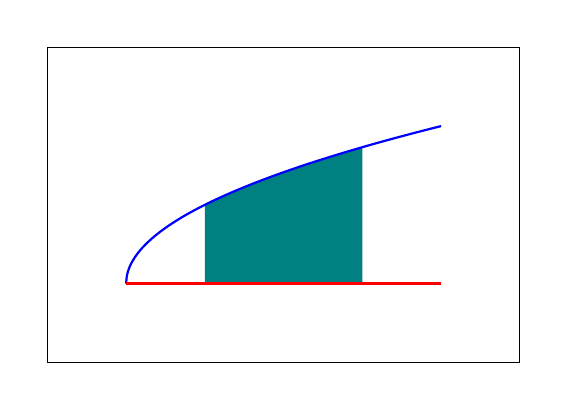
\begin{tikzpicture}
  \begin{axis}[at={(0,0)},anchor=south west,width=6cm,height=4cm,scale only axis,
    xmin=-1,xmax=5,ymin=-1,ymax=3,enlargelimits=false,axis lines=box,ticks=none]
    \addplot[blue,thick,mark=none,name path=force,domain=0:4,samples=500] {sqrt(x)};
    \draw[red,thick,name path=zero] (axis cs:0,0) -- (axis cs:4,0);
    \addplot[draw=none,fill=teal] fill between[
      of=force and zero,soft clip={(1,-0.5) rectangle (3,2.5)}];
  \end{axis}
  \path[use as bounding box] (-0.25,-0.25) rectangle (6.25,4.25);
\end{tikzpicture}
\end{document}
